\chapter{Estudi Econòmic} \label{cap:economic}

En aquest capítol s'especifiquen les despeses de desenvolupament derivades de la realització
del rootkit portat a terme en aquest projecte. Aquestes despeses fan referència només al cost humà que
ha suposat, ja que pel què fa al material de treball utilitzat, s'ha utilitzat només material del què
ja es disposava prèviament. \\

\section{Canvis en la planificació}

Primer de tot ens cal tenir clar el temps que finalment s'ha tardat en realitzar el projecte. Sabíem 
que la recerca tenia un paper molt important en el projecte i que això podia provocar alguns canvis 
en quant a les funcionalitats finals. Així ha estat. \\

Sobre la planificació inicial hi han agut principalment els següents canvis:

\begin{itemize}
    \item Eliminació de la injecció de codi en memòria de kernel (Es va eliminar ja que en kernels actuals ja no 
        és factible, i per tant es va decidir potenciar altres punts. Tot i això s'ha documentat el què i el perquè).
    \item Falta de previsió ja que inicialmet no es varen tenir en compte els períodes d'examens finals i de 
		vacances.
	\item Necessitat de molt més testeig.
\end{itemize}

Com a comentaris importants, dir que la planificació inicial es va veure força afectada a partir de la tercera setmana de Juny, que al apropar-se
examens i entregues finals d'altres assignatures, es va pactar amb el tutor per a fer una petita pausa. \\

L'altre motiu pel qual s'ha acabat allargant una mica més, ha estat la necessitat de dedicar moltes més hores per a 
deixar el rootkit amb l'estabilitat de funcionament desitjada. Totes aquestes funcionalitats programades a tant 
baix nivell (utilitzant llenguatge ensamblador en varis casos) han hagut de ser molt testejades i millorades per a
acabar obtenint un producte de qualitat. \\

Un cop aplicats els diferents canvis que han afectat el projecte, la planificació final ha estat la següent: \\
\\
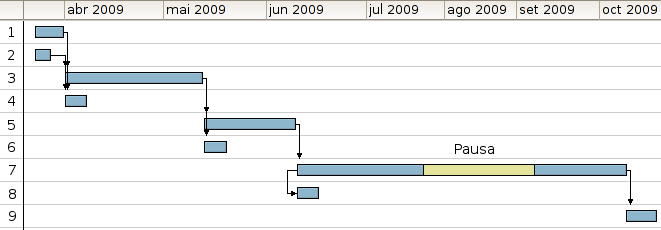
\includegraphics[scale=0.68,keepaspectratio]{segon_gantt.png} 

El principal canvi que es pot apreciar en quant a funcionalitats, és el fet de la substitució de la tasca 
d'injecció de codi en memòria del kernel, per una altre tasca de funcionalitats.

\begin{enumerate}
    \item Estructura i disseny del rootkit
    \item Estructura de la documentació
    \item Implementació de les funcionalitats bàsiques
    \item Documentació de les funcionalitats bàsiques
    \item Implementació de les funcionalitats avançades I
    \item Documentació de les funcionalitats avançades I
    \item Implementació de les funcionalitats avançades II\\
		En aquesta tasca, es varen afegir les següents funcionalitats:
		\begin{itemize}
			\item Proxy socks
			\item Mode de comunicació RAW
		\end{itemize}
    \item Documentació de les funcionalitats avançades II
    \item Anàlisi general i retocs finals
\end{enumerate}

\section{Perfils i assignació de tasques}

Per tal de quantificar el cost dels recursos humans, primer ens cal dividir els diferents participants
segons el rol que han portat a terme. En el nostre projecte, hi han participat els següents rols.

\begin{itemize}
\item Investigador \\
	Aquest perfil té la funció de proporcionar les tècniques necessàries per a cada funcionalitat, així 
	com marcar l'esquelet del rootkit. Pel què fa a les tasques del projecte, aquest perfil participa 
	en molt poca instància en les de estructura i disseny del rootkit així com a les dues tasques de
	implementació.
\item Analista / dissenyador \\
	Donades les pautes marcades per l'investigador, l'analista té la funció de definir totalment el 
	rootkit. Aquest perfil és qui completarà l'estructura i el disseny del rootkit, i especificarà 
	les diferents funcionalitats. Aquest perfil també serà el responsable de completar la part del 
	disseny contemplada en la documentació.
\item Programador \\
	El perfil de programador, és el qui ha d'acabar implementant el què l'analista ha cregut convenient.
	Aquest perfil serà el que portarà a terme majoritàriament les tasques d'implementació de funcionalitats
	així com la part de documentació de la solució.
\end{itemize}

Com es pot veure, en el nostre cas no s'assignen tasques completes a un perfil, sinó que les tasques
requereixen de un o varis perfils per a completar-se. \\

A continuació es mostra el detall d'hores d'aquesta assignació:

\subsection{Investigador}

\begin{center}
\begin{tabular}[c]{|p{12.0cm}|r|}
	\hline
	\cellcolor[gray]{0.9} {\bfseries Tasques}  & \cellcolor[gray]{0.9} {\bfseries Hores} \\
	\hline 
	Estructura i disseny del rootkit &  25 \\
	\hline Implementaci\'o de les funcionalitats b\`asiques & 10 \\
	\hline Implementaci\'o de les funcionalitats avan\c{c}ades I & 15 \\
	\hline Implementaci\'o de les funcionalitats avan\c{c}ades II & 20 \\
	\hline An\`alisi general i retocs finals & 100 \\
	\hline 
\end{tabular}
\end{center}

\subsection{Analista / dissenyador}

\begin{center}
\begin{tabular}[c]{|p{12.0cm}|r|}
	\hline 
	\cellcolor[gray]{0.9} {\bfseries Tasques} & \cellcolor[gray]{0.9} {\bfseries Hores} \\
	\hline Estructura i disseny del rootkit &  30  \\
	\hline Estructura de la documentaci\'o &  10  \\
	\hline Implementaci\'o de les funcionalitats b\`asiques & 10 \\
	\hline Documentaci\'o de les funcionalitats b\`asiques & 10  \\
	\hline Implementaci\'o de les funcionalitats avan\c{c}ades I & 10 \\
	\hline Documentaci\'o de les funcionalitats avan\c{c}ades I & 10  \\
	\hline Implementaci\'o de les funcionalitats avan\c{c}ades II & 10 \\
	\hline Documentaci\'o de les funcionalitats avan\c{c}ades II & 10 \\
	\hline An\`alisi general i retocs finals & 20  \\
	\hline
\end{tabular}
\end{center}

\subsection{Programador}

\begin{center}
\begin{tabular}[c]{|p{12.0cm}|r|}
	\hline
	\cellcolor[gray]{0.9} {\bfseries Tasques} & \cellcolor[gray]{0.9} {\bfseries Hores} \\
	\hline Implementaci\'o de les funcionalitats b\`asiques & 230  \\
	\hline Documentaci\'o de les funcionalitats b\`asiques &  15  \\
	\hline Implementaci\'o de les funcionalitats avan\c{c}ades I & 160  \\
	\hline Documentaci\'o de les funcionalitats avan\c{c}ades I & 15 \\
	\hline Implementaci\'o de les funcionalitats avan\c{c}ades II & 350 \\
	\hline Documentaci\'o de les funcionalitats avan\c{c}ades II & 15 \\
	\hline An\`alisi general i retocs finals & 80 \\
	\hline
\end{tabular}
\end{center}


\section{Càlcul de costos}

Per tal de poder quantificar el cost, ha estat necessari estimar un preu hora per
cadascun dels perfils. Així doncs, s'ha considerat que el preu hora de l'investigador és de 85\euro/h,
el del analista és de 65\euro/h i el del programador de 45\euro/h. \\

Amb aquests costos i l'assignació de tasques anterior, podem calcular un cost total del projecte de:

\begin{figure}[htp]
\centering
\begin{tabular}{c c c c}
	\textbf{Perfil} & \textbf{Hores} & \textbf{Preu hora} & \textbf{Preu total} \\
	\hline
	Investigador & 170 & 85\euro & 14.450\euro \\
	Analista & 120 & 65\euro & 7.800\euro \\
	Programador & 865 & 45\euro & 38.925\euro \\
	& & \textbf{Total} & 61.175\euro \\
\end{tabular}
\caption{Cost total del projecte}
\label{fig:costProjecte}
\end{figure}

